\documentclass[preview]{standalone}

\usepackage{amsmath}
\usepackage{amssymb}
\usepackage{stellar}
\usepackage{definitions}
\usepackage{tikz}
\usetikzlibrary{decorations.markings}

\begin{document}

\id{thermodynamics-exercises}
\genpage

\section{Esercises}

\begin{snippetexercise}{thermodynamics-ex-1}{}
    Two metal rods are aligned at one end and bolted together. Knowing that the coefficients of thermal expansion are respectively
    \[
    \lambda_1 = 1.9 \times 10^{-5}\, ^\circ\text{C}^{-1}, \quad 
    \lambda_2 = 1.1 \times 10^{-5}\, ^\circ\text{C}^{-1},
    \]
    and that the shorter rod at \(0^\circ\text{C}\) is \(2.2\,\text{m}\) long, calculate the length at \(0^\circ\text{C}\) of the second rod such that the difference
    \(\Delta L = \text{constant}\), despite large variations in temperature.
\end{snippetexercise}

\begin{snippetsolution}{thermodynamics-ex-1-sol}{}
    Let \(l_1\) and \(l_2\) be the respective lengths at \(0^\circ\text{C}\).
    The difference is given by
    \begin{align*}
        \Delta L(T) &= l_1 + l_1 \lambda_1 (T - 0) - \left( l_2 + l_2 \lambda_2 (T - 0) \right) \\
        &= l_1 + l_2 + T\left(l_1 \lambda_1 - l_2 \lambda_2\right)
    \end{align*}
    since this needs to be constant, the temperature dependence must vanish:
    \begin{align*}
        l_1 \lambda_1 - l_2 \lambda_2 &= 0 \\
        l_2 &= \frac{\lambda_1}{\lambda_2}l_1
    \end{align*}
\end{snippetsolution}

\begin{snippetexercise}{thermodynamics-ex-2}{}
    A mass \(m_1 = 15\ \text{g}\) of \( \text{N}_2 \)
    (molar mass \(M_{\text{N}_2} = 28\ \text{g/mol}\)) and a mass
    \(m_2 = 20\ \text{g}\) of \( \text{O}_2 \) (molar mass \(M_{\text{O}_2} = 32\ \text{g/mol}\)) are mixed in a cylinder closed by
    a frictionless sliding piston.
    Find the partial pressures of the two gases (assumed ideal) when the external pressure is \(1\ \text{atm}\).
\end{snippetexercise}

\begin{snippetsolution}{thermodynamics-ex-2-sol}{}
    \todo
\end{snippetsolution}

\begin{snippetexercise}{thermodynamics-ex-3}{}
    A monoatomic ideal gas with \(n = 1\,\text{mol}\) is compressed at constant pressure \(p = 2\,\text{atm}\) from \(V = 10\,\text{L}\) to \(V = 2\,\text{L}\). It then undergoes an isochoric transformation, followed by an isothermal transformation returning to the initial state. Calculate the work done and the heat absorbed during the cycle.

    \begin{center}
    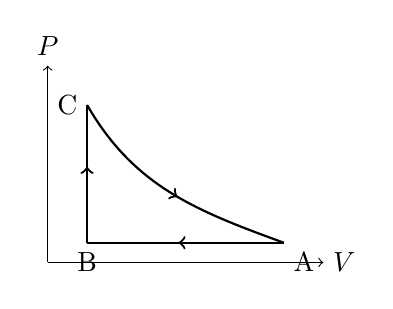
\begin{tikzpicture}[scale=0.5]
    \draw[->] (0,0) -- (7,0) node[right] {$V$};
    \draw[->] (0,0) -- (0,5) node[above] {$P$};

    % points
    \coordinate (A) at (6,0.5); % bottom right
    \coordinate (B) at (1,0.5); % bottom left
    \coordinate (C) at (1,4);   % top left

    % cycle lines (with mid arrows)
    \draw[thick,postaction={decorate},
        decoration={markings, mark=at position 0.5 with {\arrow{<}}}] 
        (A) to[out=160,in=300] (C); % A->C

    \draw[thick,postaction={decorate},
        decoration={markings, mark=at position 0.5 with {\arrow{<}}}] 
        (C) -- (B); % C->B

    \draw[thick,postaction={decorate},
        decoration={markings, mark=at position 0.5 with {\arrow{<}}}] 
        (B) -- (A); % B->A

    % labels
    \node[left] at (C) {C};
    \node[below] at (B) {B};
    \node[below right] at (A) {A};

    \end{tikzpicture}
    \end{center}
\end{snippetexercise}

\begin{snippetsolution}{thermodynamics-ex-3-sol}{}
    \todo
\end{snippetsolution}

\begin{snippetexercise}{thermodynamics-ex-4}{}
    \todo
\end{snippetexercise}

\begin{snippetsolution}{thermodynamics-ex-4-sol}{}
    \todo
\end{snippetsolution}

\begin{snippetexercise}{thermodynamics-ex-5}{}
    \todo
\end{snippetexercise}

\begin{snippetsolution}{thermodynamics-ex-5-sol}{}
    \todo
\end{snippetsolution}

\begin{snippetexercise}{thermodynamics-ex-6}{}
    \todo
\end{snippetexercise}

\begin{snippetsolution}{thermodynamics-ex-6-sol}{}
    \todo
\end{snippetsolution}

\begin{snippetexercise}{thermodynamics-ex-7}{}
    \todo
\end{snippetexercise}

\begin{snippetsolution}{thermodynamics-ex-7-sol}{}
    \todo
\end{snippetsolution}

\begin{snippetexercise}{thermodynamics-ex-8}{}
    \todo
\end{snippetexercise}

\begin{snippetsolution}{thermodynamics-ex-8-sol}{}
    \todo
\end{snippetsolution}

\begin{snippetexercise}{thermodynamics-ex-9}{}
    \todo
\end{snippetexercise}

\begin{snippetsolution}{thermodynamics-ex-9-sol}{}
    \todo
\end{snippetsolution}

\end{document}